%% LaTeX-Beamer template for KIT design
%% by Erik Burger, Christian Hammer
%% title picture by Klaus Krogmann
%%
%% version 2.1
%%
%% mostly compatible to KIT corporate design v2.0
%% http://intranet.kit.edu/gestaltungsrichtlinien.php
%%
%% Problems, bugs and comments to
%% burger@kit.edu

\documentclass[18pt]{beamer}

\usepackage[utf8]{inputenc}
\usepackage[babel,german=quotes]{csquotes}
\usepackage{graphicx}
\usepackage{caption}
\usepackage{subfig}
\usepackage[right]{eurosym}
\usepackage{listings}

%% SLIDE FORMAT

% use 'beamerthemekit' for standard 4:3 ratio
% for widescreen slides (16:9), use 'beamerthemekitwide'

\usepackage{templates/beamerthemekit}
% \usepackage{templates/beamerthemekitwide}

%% TITLE PICTURE

% if a custom picture is to be used on the title page, copy it into the 'logos'
% directory, in the line below, replace 'mypicture' with the 
% filename (without extension) and uncomment the following line
% (picture proportions: 63 : 20 for standard, 169 : 40 for wide
% *.eps format if you use latex+dvips+ps2pdf, 
% *.jpg/*.png/*.pdf if you use pdflatex)

\titleimage{title}

%% TITLE LOGO

% for a custom logo on the front page, copy your file into the 'logos'
% directory, insert the filename in the line below and uncomment it

\titlelogo{titlelogo}

% (*.eps format if you use latex+dvips+ps2pdf,
% *.jpg/*.png/*.pdf if you use pdflatex)

%% TikZ INTEGRATION

% use these packages for PCM symbols and UML classes
% \usepackage{templates/tikzkit}
% \usepackage{templates/tikzuml}

% the presentation starts here

\title[C++ Workshop]{C++ Workshop}
\subtitle{1. Block, 27.04.2012}
\author{Markus Jung, Christian Käser, Robert Schneider}

\institute{}

\begin{document}

% change the following line to "ngerman" for German style date and logos
\selectlanguage{ngerman}

%title page
\begin{frame}
\titlepage
\end{frame}

%table of contents
\begin{frame}{Gliederung}
\tableofcontents
\end{frame}

\section{Versionsverwaltung}
\subsection{Motivation}
\begin{frame}{Motivation}
	\begin{itemize}
		\item \enquote{Gestern ging es noch \dots}
		\item \enquote{Das Problem hatten wir doch schon Mal \dots}
		\item \enquote{Wer hat den ?\&(\%!\$ verzapft!?}
	\end{itemize}
	\ \\
	\pause
	\ \\
	\begin{block}{Aufgaben}
		\begin{itemize}
			\item Archivierung der Entwicklungsgeschichte
			\begin{itemize}
				\item \enquote{Zeitmaschine}
			\end{itemize}
			\item Koordination paralleler Entwicklungsvorgänge
		\end{itemize}
	\end{block}
\end{frame}

\subsection{Konzepte}
\begin{frame}{Konzepte I}
	\begin{block}{Version/Revision}
		Eine Momentaufnahme der verwalteten Dateien, verknüpft mit Metadaten wie Autor oder Datum
	\end{block}
	\begin{block}{Versionsgeschichte}
		Stellt den Bezug zwischen einzelnen Versionen her
	\end{block}
	\begin{block}{Repository}
		Speichert und verwaltet die Versionsgeschichte sowie die zugehörigen Versionen
	\end{block}
	\begin{block}{Arbeitskopie}
		Ein Abbild einer Version im Dateisystem, an dem auch Änderungen vorgenommen werden können
	\end{block}
\end{frame}
\begin{frame}{Konzepte I}
	\begin{figure}
		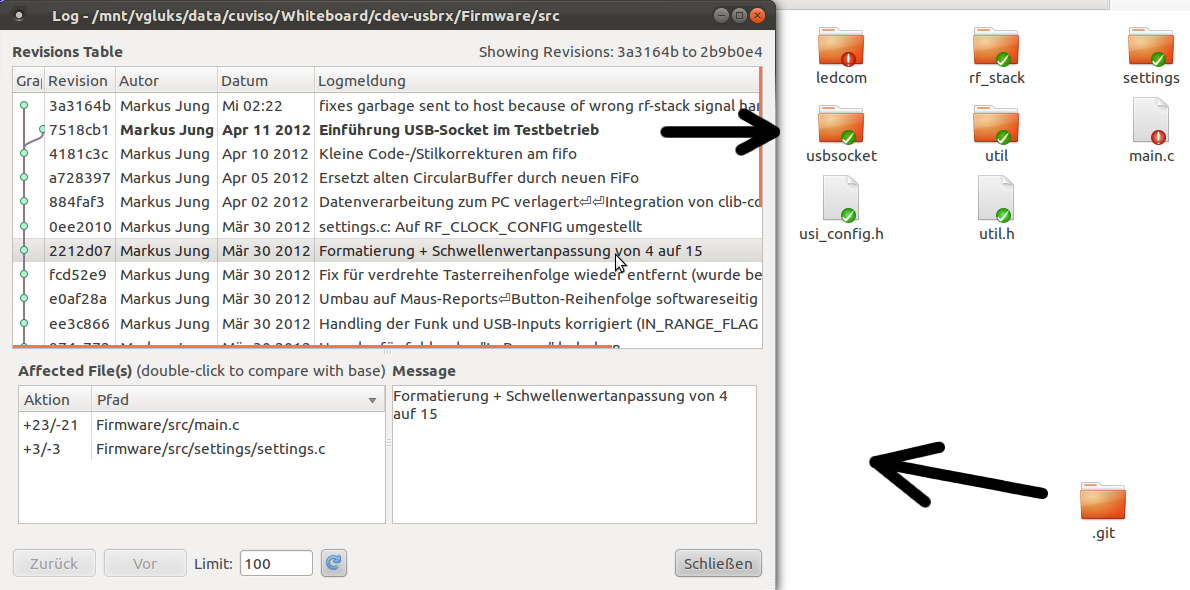
\includegraphics[width=\linewidth]{images/history.png}
	\end{figure}
\end{frame}
\begin{frame}{Konzepte II}
	% parallele entwicklung: branch, merge, tag
	\begin{columns}
		\column{.1\linewidth}
			\begin{figure}
				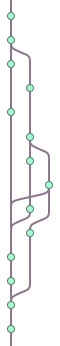
\includegraphics[width=\linewidth]{images/branchmerge.png}
			\end{figure}

		\column{.9\textwidth}
			\begin{block}{Branch}
				\begin{itemize}
					\item Softwareentwicklung ist selten linear (\enquote{Entwicklungszweig})
					\item Versionsverwaltungen bilden das durch \enquote{branches} ab
				\end{itemize}
			\end{block}
			\begin{block}{Merge}
				\begin{itemize}
					\item Führt Entwicklungszweige zusammen
					\item Konkurrierende Änderungen können Konfliktlösung erfordern
				\end{itemize}
			\end{block}
			\begin{block}{Tag}
				Markiert Versionen zum schnellen Zugriff
			\end{block}
	\end{columns}
\end{frame}

\begin{frame}{Zentral vs. Dezentral}
	\begin{block}{Zentral}
		Es gibt nur ein Repository über das alle Aktivitäten abgewickelt werden
		\begin{itemize}
			\item Erfordert möglichst kontinuierlichen Zugriff auf den Server
			\item Zentrale Anlaufstelle, damit auch: Konflikt-Brennpunkt
			\item Vertreter: RCS, CVS, SVN, Visual Source Safe
		\end{itemize}
	\end{block}
	\begin{block}{Dezentral}
		Jeder Nutzer hat ein (lokales) Repository, Änderungen werden zwischen Repositorys ausgetauscht
		\begin{itemize}
			\item Erfordert keinen kontinuierlichen Zugriff auf den Server
			\item Verschiedene Sichtweisen des gleichen Entwicklungsvorgangs
			\item Lokales Repository $\rightarrow$ Lokaler Namensraum
			\item Vertreter: GIT, Mercurial, Bazaar
		\end{itemize}
	\end{block}
\end{frame}

\subsection{GIT}
\begin{frame}{GIT}
\end{frame}

\begin{frame}{GIT Workflow}
% GIT Workflow: init/clone/checkout/commit/pull/push/branch/merge
\end{frame}

\begin{frame}{GIT und github}
% Github: fork/pullreq
\end{frame}

\subsection{Weiterführende Hinweise}
\begin{frame}{Hilfe zur Selbsthilfe}
% Verweis auf die Hilfe zur Selbsthilfe
\end{frame}

\subsection{Aufgaben}
\begin{frame}{Aufgaben}
% Aufgaben
\end{frame}

\appendix
\beginbackup

\begin{frame}[allowframebreaks]{Links}
\end{frame}

\backupend

\end{document}
